\section{Описание}
Требуется написать реализацию алгоритма поразрядной сортировки для упорядочивания пар \enquote{ключ-значение} по возрястанию.

Как сказано в \cite{Kormen}: \enquote{Поразрядная сортировка - это алгоритм, который использовался в машинах, предназначеных для сортировки перфокарт,
состоящих из d-значных чисел. 
Сначала производится сортировка по младшей цифре, после чего перфокарты снова объединяются в одну колоду,
 в которой сначала идут перфокарты из нулевого приемника, затем — из
первого приемника, затем — из второго и т.д. После этого вся колода снова сортируется по предпоследней цифре,
 и перфокарты вновь собираются в одну стопку
тем же образом. Процесс продолжается до тех пор, пока перфокарты не окажутся отсортированными по всем d цифрам. 
После этого перфокарты оказываются
полностью отсортированы в порядке возрастания d-значных чисел. Таким обра
зом, для сортировки перфокарт требуется лишь d проходов колоды.
Ниже представлен пример использования данного алгоритма для сортировки 3-х значныйх чисел.\\
\\
\textbf{Важно, чтобы сортировка по цифрам того или иного разряда в этом алгоритме
обладала устойчивостью!}}.

% надо с размерами поиграть
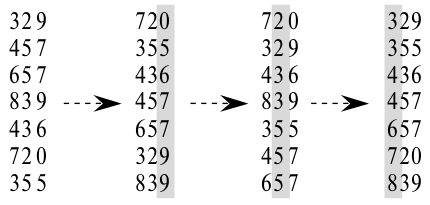
\includegraphics{src/radix_sort_impl.png}

\pagebreak

\section{Исходный код}
% Здесь должно быть подробное описание программы и основные этапы написания кода.

На каждой непустой строке входного файла располагается пара \enquote{ключ-значение}, поэтому создадим новый 
объект класса $TObject$, в которой будем хранить ключ и значение. У этого класса реализованы коснструкторы и деструкторы, 
а также переопределен опрератор присваивания и оператор вывода.


\begin{itemize}
	\item TObject() - дефолтный конструктор, по сути собирает простую пару, где ключ равен 0, а занчение это нулевой указатель
	\item TObject(key, value) - конструктор, на который принимает ключ и значение
	\item TObject(TObject \& other) - копирующий конструктор
	\item ~TObject() - деструктор
	\item operator= - оператор присваивания
	\item operator<< - опрератор вывода
\end{itemize}


Важно отметить, что в поле значения класса $TObject$ лежит указатель на строку. Как показали тесты, 
такой способ хранения строк помогает расходовать меньше памяти во время выполенения алгоритма сортировки.
При обработке вектора в процессе сортировки происходит перемещение элементов из одного вектора в другой, 
а также элементы перемещаются из одного буфера в другой при расширении или сужения буфера. 
Если хранить в поле класса сами строки, то программа будет использовать больше памяти и времени.\\\\

Нам нужно где-то хранить наши объекты, чтобы их можно было отсортировать и вывести. Так как мы не знаем, 
сколько пар поступит на вход программе, нужно использовать структуру, которая может граммотно изменять размеры своего буфера.
В ходе лабораторной работы зарпещено использовать \enquote{stl} контейнеры. Поэтому напишем свой \enquote{простой} вектор.
Этот контейнер отдаленно напоминает стандартный вектор. В нем есть такие методы, как:\\

\begin{itemize}
	\item PushBack - вставка элемента в конец буфера
	\item PopBack - удаление элемента из конца буфера
	\item Size - возвращает значение длины вектора
	\item Reserve - выделение памяти
	\item operator[] - получение элемента по индексу
	\item operator \(<<\) - печать объектов вектора
\end{itemize} 


Данный вектор написан в виде шаблонного класса $TSimpleVector$. В этом классе есть также конструкторы и деструктор.

\begin{itemize}
	\item TSimpleVector() - дефолтный конструктор
	\item TSimpleVector(const int \& n) - конструктор, который выделяет буфер на $n$ значений
	\item TSimpleVector(const int \& n, const T \& value) - конструктор, который выделяет буфер на $n$ значений и заполняет его значениями value
	\item TSimpleVector(TSimpleVector<T>\&\& other) - перемещающий конструктор (move constructor)
	\item ~TSimpleVector() - деструктор, специальный метод класса, который автоматически вызывается при уничтожении объекта. Он используется для освобождения ресурсов, выделенных объектом во время его жизни.
\end{itemize}


\textbf{Конструктор перемещения} - это специальный конструктор класса, который принимает временный объект (rvalue) 
в качестве параметра и перемещает его ресурсы в новый объект, вместо их копирования.

Важным методом нашего вектора является метод $Reserve$. У вектора есть три парамметра: размер, объем и буфер. 
В данный метод позволяет изменять объем буфера. Когда нам важно изменять объем буфера?

В основном, когда размер вектора равен объему. В стандартном векторе используются сложные конструкции, чтобы максимально экономно расходовать память.
В нашем же случае сложные конструкции пока не известны нам, поэтому мы просто стараемся увеличивать объем в 2 раза.

При выполнении лабораторной работы не использовал метод $PopBack$, но в нем тоже реализован механизм уменьшения памяти.\\\\

С хранением элементов разобрались, теперь рассмотрим алгоритм сортировки.

Почему поразрядная сортировка? Потому что сортируются разряды чисел.

Поразрядная сортировка в нашей реализации состоит из двух частей: \\

\begin{itemize}
	\item функция для получения разряда числа $GetDigit$
	\item сортировка разрядов
\end{itemize}

Для хранения ключа используется тип данных $uint64_t$ - 8 байт.
Для получения разряда не нужно использовать деление на 10 и деление с остатком. Этот способ работает, 
но он для больших чисел он будет неэффективным. Поэтому нужно разбить число на байты. Можно сравнить два подхода.
В функции поразрядной сортировки запускаем сотировку разрядов в цикле. Цикл можем запустить от 0 до 14 или от 0 до 8.
Очевидно, что второй вариант более привлекателен с точки зрения экономии ресурсов.

Внутри функции $GetDigit$ выполняется следующее:
\begin{enumerate}
	\item Сдвиг числа elem на 8 * i битов вправо с помощью оператора \(>>\). Это позволяет получить нужную позицию цифры в числе.
	\item Применение побитовой маски 0xFF с помощью оператора \&. Маска 0xFF представляет \textbf{байт} со значением 255 в двоичной системе. Применение этой маски позволяет извлечь только младший байт (8 бит) из результата сдвига, что соответствует значению цифры.
	\item Полученное значение цифры сохраняется в переменную $digit$.
	\item Функция возвращает значение $digit$.
\end{enumerate}


Как уже описывалось выше, разряды чисел должны сортироваться устойчивой сотртировкой. Мы будем использовать сортировку подсчетом.\\\\

Приведем краткий разбор алгоритма по шагам.
\begin{enumerate}
	\item создание массива подсчета
	\item вычисление префикс-суммы для каждого элемента в массиве подсчета
	\item создание результырующего вектора
	\item вычисление позиции ткущего элемента в результирующем векторе
\end{enumerate}


Алгоритм сортировки посчетом достаточно прост. Нужно создать массив подсчета, 
куда будем записывать количество элемнетов которые нам повстречались при обходе.
В нашем случае такой массив может быть максимум размером 256 элементов, что соотвествуент 1 байту.
Поэтому нет смысла использовать наш вектор.\\\\

После нужно вычислить префикс-суммы для каждого значения в массиве подсчета, начиная со 2 элемента.
Данная префикс-сумма обозначает количество элементов, которые меньше или равны текущему элементу и стоят где-то перед ним.
Поэтому и начинаем со второго элемента, перед первым ничего не стоит.

Далее нам нужен результирующий вектор, куда мы будем помещать элементы. 

В сортировки подсчетом нет сравнения элементов. Элементы сортируются за счет вычисления их позиции в результирующем векторе.
Позиция вычисляется как значение массива подсчета (от текущего разряда) минус 1.

На вычесленную позицию ставим элемент исходного вектора и уменьшаем значение в массиве подсчета.

Важно отметить, что для расстановки элементов в результирующем векторе цикл запускают от последнего элемента к первому.
Именно так можно расставить элементы в правильном порядке, как раз для этого мы вычисляли префикс-сумму.

После выполенения цикла, перемещаем новую последовательность из результирующего вектора в исходный.

После того как выполним 8 раз порязрядную сортировку, наша исходная последовательность будет упорядочена по возрастанию.


Чтобы программа не превысила времени выполнения, придется переписать ввод и вывод пар. Вместо использования cin  и cout,
бедем использовать scanf и printf.\\\\


\begin{lstlisting}[language=C]
#include <iostream>
#include <memory>

template<class T>
class TSimpleVector {
    private:
        T* buffer;
        int size;
        int cap;
    public:
        TSimpleVector();
        TSimpleVector(const int & n);
        TSimpleVector(const int & n, const T & value);
        TSimpleVector(TSimpleVector<T>&& other); // move constructor
        ~TSimpleVector();

        void Reserve(const int new_cap)
        void PushBack(const T & value);
        void PopBack();
        int Size() const; // getter

        T& operator[](const int & i);
        TSimpleVector& operator=(TSimpleVector<T>&& other);
        
        friend std::ostream& operator<<(std::ostream& os, const TSimpleVector<T>& other);
};

class TObject {
    public:
        uint64_t key;
        std::shared_ptr<std::string> value;

        TObject();
        TObject(const uint64_t& c_key, const std::string& c_value);
        TObject(const TObject& other);
        ~TObject() noexcept;

        TObject& operator=(const TObject& other);
        friend std::ostream& operator<<(std::ostream& os, const TObject & other);
};

const int COUNT_MS_SZ = 256;

int GetDigit(uint64_t & elem, int& i) {
	int digit = (elem >> (8 * i)) & 0xFF;
	return digit;
}

void CountingSort(TSimpleVector<TObject>& mas, int& i) {
	int sz = mas.Size();
	int cnts[COUNT_MS_SZ] = {0};

	for (int j = 0; j < sz; j++) {
		cnts[GetDigit(mas[j].key, i)]++;
	}

	for (int j = 1; j < COUNT_MS_SZ; j++) {
		cnts[j] += cnts[j - 1];
	}

	TSimpleVector<TObject> interm_result(sz);

	for (int j = sz - 1; j >= 0; j--) {
		int pos = cnts[GetDigit(mas[j].key, i)] - 1;
		interm_result[pos] = mas[j];
		cnts[GetDigit(mas[j].key, i)] = pos;
	}

	mas = std::move(interm_result);
}

void Radix(TSimpleVector<TObject>& mas) {
	for (int i = 0; i < 8; i++) {
		CountingSort(mas, i);
	}
}

int main() {
	TSimpleVector<TObject> mas;

	uint64_t key;
	char str[2049];
	while (scanf("%lu\t%[^\n]", &key, str) != EOF) {
		mas.PushBack(TObject(key, std::string(str)));
	}

	Radix(mas);

	for (int i = 0; i < mas.Size(); i++) {
		printf("%lu\t%s\n", mas[i].key, mas[i].value->c_str());
	}

}
	
	
\end{lstlisting}

% В случае, если код не помещается на одну-две страницы $A4$, тогда следует сделать табличку следующего вида:
% \begin{longtable}{|p{7.5cm}|p{7.5cm}|}
% \hline
% \rowcolor{lightgray}
% \multicolumn{2}{|c|} {main.c}\\
% \hline
% void sort(struct KV \& B, struct KV \& Res, int max, int size)&Функция сортировки подсчётом\\
% \hline
% \rowcolor{lightgray}
% \multicolumn{2}{|c|} {file1.c}\\
% \hline
% void function\_name()&Функция, \enquote{которая почти всегда работает, но неясно, что она делает}.\\
% \hline
% \end{longtable}
% В этом случае структуры или классы должны быть полностью приведены в листинге (без реализации методов).
% \begin{lstlisting}[language=C]
% struct KV{
% 	int key;
% 	char value;
% } KV;
% \end{lstlisting}
\pagebreak

\section{Консоль}
\begin{alltt}
alex@wega:~/da_labs/Lab_01$ make
g++ -std=c++17 -pedantic -Wall main.cpp -o lab1
alex@wega:~/da_labs/Lab_01$ cat tests/01.t
17832977662492897515    lMlOCeWaHK
2996444704890835419     eoRbLbhgnV
14252360749301456558    XViwJgagyL
8509929984979068612     lEPeVZQJxj
16872145630083976482    OzbvidEVHy
12066295488853181134    BfJiYdMhdv
4473799090154691171     RHxbAUdqfb
1681540776916609004     EGLTpVNggw
5616851010130146808     xlYdMhNVCa
6958989457477228380     mXzlaEkRSD
alex@wega:~/da_labs/Lab_01$ ./lab1 < tests/01.t
1681540776916609004     EGLTpVNggw
2996444704890835419     eoRbLbhgnV
4473799090154691171     RHxbAUdqfb
5616851010130146808     xlYdMhNVCa
6958989457477228380     mXzlaEkRSD
8509929984979068612     lEPeVZQJxj
12066295488853181134    BfJiYdMhdv
14252360749301456558    XViwJgagyL
16872145630083976482    OzbvidEVHy
17832977662492897515    lMlOCeWaHK

alex@wega:~/da_labs/Lab_01$ make
g++ -std=c++17 -pedantic -Wall main.cpp -o lab1
alex@wega:~/da_labs/Lab_01$ cat tests/01.t
31      G
10      h
86      T
23      x
33      U
59      s
37      K
28      e
16      V
100     P
alex@wega:~/da_labs/Lab_01$ ./lab1 < tests/01.t
10      h
16      V
23      x
28      e
31      G
33      U
37      K
59      s
86      T
100     P

alex@wega:~/da_labs/Lab_01$ make
g++ -std=c++17 -pedantic -Wall main.cpp -o lab1
alex@wega:~/da_labs/Lab_01$ cat tests/01.t
44      vADburXqfnTEriMoBSYX
53      fsyBYfJCGcmDRfUyEyKe
0       XEvKskWSoFDjdhrFTBtn
81      BxmBxxSFIAdkdFtZBtaz
87      bqjHGUGbjkMFmYWtJKSP
58      ZGxZTCJICBOHqnmGMXTl
74      NtEemPdRbdbybJMyfhMP
86      sXCpqkqXiBKLhmbyMXKX
41      dUwSlJRZtsodWiZTLNVn
24      tKNWPsWSuvPxydjtcAeM
alex@wega:~/da_labs/Lab_01$ ./lab1 < tests/01.t
0       XEvKskWSoFDjdhrFTBtn
24      tKNWPsWSuvPxydjtcAeM
41      dUwSlJRZtsodWiZTLNVn
44      vADburXqfnTEriMoBSYX
53      fsyBYfJCGcmDRfUyEyKe
58      ZGxZTCJICBOHqnmGMXTl
74      NtEemPdRbdbybJMyfhMP
81      BxmBxxSFIAdkdFtZBtaz
86      sXCpqkqXiBKLhmbyMXKX
87      bqjHGUGbjkMFmYWtJKSP
alex@wega:~/da_labs/Lab_01$
\end{alltt}
\pagebreak
